\documentclass[12pt]{article}
\usepackage[pdftex]{graphicx}
\usepackage{amsmath}
\usepackage{hyperref}
\usepackage{alltt}
\usepackage{pgfplots}
\usepackage{circuitikz}
\usepackage{tikz}
\usetikzlibrary{arrows.meta}
\usepackage{tikz-3dplot}

% Define a custom command for TikZ
\newcommand{\myTikZ}{Ti\textit{k}Z }


\begin{document}
\section{Punto 1}

Escribe un script \myTikZ que dibuje un triángulo rectángulo con vértices $(0,0), (4,0), (0,3)$.
Calcula, usando el teorema de Pitágoras, la longitud de la hipotenusa y escribe esto
en un texto encima de la hipotenusa inclinada para que quede paralela a ella.
Escribe también el ángulo en el vértice $(4,0)$. En otras palabras, escribe un guión que
muestra la siguiente figura.

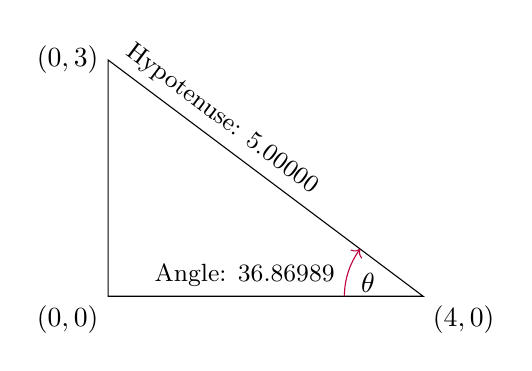
\begin{tikzpicture}
    \coordinate (A) at (0,0);
    \coordinate (B) at (0,3);
    \coordinate (C) at (4,0);
    
    \draw (A) -- (B) -- (C) -- cycle;
    
    \pgfmathsetmacro{\sideA}{3}
    \pgfmathsetmacro{\sideB}{4}
    \pgfmathsetmacro{\hypotenuse}{sqrt(\sideA^2 + \sideB^2)}
    

    \node[below left] at (A) {$(0,0)$};
    \node[left] at (B) {$(0,3)$};
    \node[below right] at (C) {$(4,0)$};
    

    \pgfmathsetmacro{\angle}{atan(\sideA/\sideB)}

    \node[above right, rotate=-\angle] at (B) {\small Hypotenuse: $\hypotenuse$};
    \node[above left, xshift=-1cm] at (C) {\small Angle: $\angle$};



    \pgfmathsetmacro{\startAngle}{180}  % units of degrees
    \pgfmathsetmacro{\endAngle}{180-\angle}
    \pgfmathsetmacro{\R}{1.0}  % units of points
    \coordinate (A) at (3,0);
     \draw[->, purple] (A) 
       arc (\startAngle:\endAngle:\R); 

    \node [above, yshift=-2pt] at (3.3,0) {$\theta$};
\end{tikzpicture}


\section{Punto 2}

Ponerle etiquetas a las dos funciones no etiquetadas en
la grafica con parabola, funcion **seno** y **exponencial**. Estas dos ultimas son las que toca etiquetar.

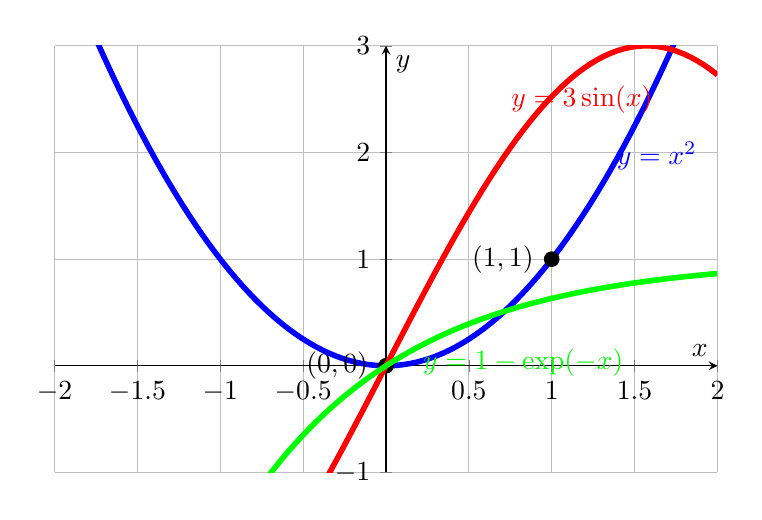
\begin{tikzpicture}
    \begin{axis}[
        axis lines=middle,
        xlabel=$x$,
        ylabel=$y$,
        xmin=-2, xmax=2,
        ymin=-1, ymax=3,
        grid=both,
        width=10cm,
        height=7cm,
        samples=100 % Number of samples for smooth curve
    ]
    
    % Plot the function
    % Function: y = x^2
    \addplot[blue, domain=-2:2, line width=2] {x^2} 
        node[pos=0.8, below right, xshift=-10pt] {$y=x^2$}; 
    
    % Mark some key points
    \node[label={180:{$(0,0)$}}, circle, fill, inner sep=2pt] at (axis cs:0,0) {};
    \node[label={180:{$(1,1)$}}, circle, fill, inner sep=2pt] at (axis cs:1,1) {};
    
    % Function: y=3 sin(x*180/pi)
    \addplot[red, line width=2,  domain=-2:2] {3*sin(x*180/pi)}
        node[pos=0.8, above right, xshift=-10pt] {$y=3\sin(x)$};
        
    % Function: y=1-exp(-x)
    \addplot[green, line width=2, domain=-2:2] {1-exp(-x)} 
        node[pos=0.8, below right, xshift=-10pt] {$y=1-\exp(-x)$};
    
    \end{axis}
\end{tikzpicture}

\section{Punto 3}

Asuma que usted es profesor de fisica y quiere ensenhar suma de vectores.
Escoja dos vectores (numericos en 3D) y haga la suma de dos formas
  * Por metodo del paralelogramo.
  * El segundo comienza en la cabeza del primero. Se forma un triangulo,
    el primero del origen a A, el segundo de A a B y la resultante del origen a B.
    La suma se hace con \myTikZ. (usando `pgfmathsetmacro`).


Metodo paralelogramo
\begin{center}
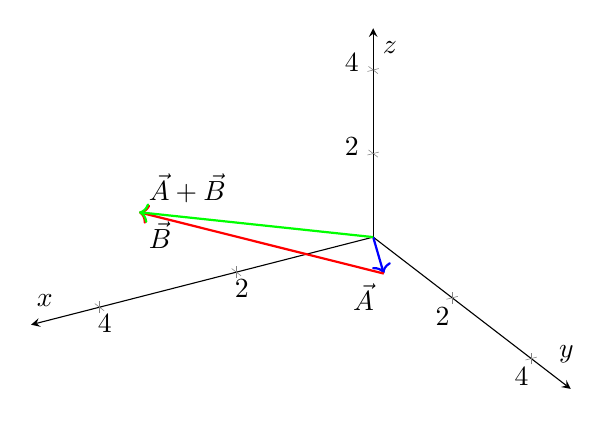
\begin{tikzpicture}
    \begin{axis}[
        view={150}{40},
        axis lines=center,
        xlabel=$x$,
        ylabel=$y$,
        zlabel=$z$,
        xmin=0, xmax=5,
        ymin=0, ymax=5,
        zmin=0, zmax=5,
        grid=major,
    ]
    \pgfmathsetmacro{\xa}{1}
    \pgfmathsetmacro{\ya}{2}
    \pgfmathsetmacro{\za}{1}
    \pgfmathsetmacro{\xb}{3}
    \pgfmathsetmacro{\yb}{-1}
    \pgfmathsetmacro{\zb}{2}
    \pgfmathsetmacro{\xr}{\xa+\xb}
    \pgfmathsetmacro{\yr}{\ya+\yb}
    \pgfmathsetmacro{\zr}{\za+\zb}
    
    % Vector A
    \addplot3[->, thick, blue] coordinates {(0,0,0) (\xa, \ya, \za)};
    \node[below left] at (axis cs:\xa, \ya, \za) {$\vec{A}$};
    
    % Vector B from end of A
    \addplot3[->, thick, red] coordinates {(\xa, \ya, \za) (\xr, \yr, \zr)};
    \node[below right] at (axis cs:\xr, \yr, \zr) {$\vec{B}$};
    
    % Vector A+B
    \addplot3[->, thick, green] coordinates {(0,0,0) (\xr, \yr, \zr)};
    \node[above right] at (axis cs:\xr, \yr, \zr) {$\vec{A} + \vec{B}$};
    
    \end{axis}
\end{tikzpicture}
\end{center}





\end{document}

